\newpage
\section{Interface client}
\subsection{Intérêt principal}
On dit souvent qu'un dessin vaut mieux qu'un long discours.
Partant de ce principe, l'objectif de Colladia est de proposer aux utilisateurs une expérience leur permettant de pouvoir dessiner, ensemble, chacun sur leur propre appareil mobile. 

Les utilisateurs peuvent ainsi modifier le document simultanément, et profiter des interactions tactiles qu'offrent ces supports.
Que ce soit en déplacement ou en réunion, il n'est pas toujours possible d'avoir un ordinateur avec soi.
Dans ce genre de situation, Colladia se révèle particulièrement intéressant. 

\subsection{Utilisateurs visés}
Les premiers utilisateurs visés seront notamment les étudiants et les professionnels qui rencontrent la nécessité de réaliser des diagrammes ou des schémas dans leur quotidien.
L'application est axée sur ces utilisateurs pour proposer des éléments de diagramme adaptés à leurs besoins.

\subsection{Étude des utilisateurs (interviews, enquêtes)}
Afin de déterminer les besoins des utilisateurs de façon pertinente, un sondage a été réalisé auprès des étudiants de l’UTC venant de diverses branches.
Les questions étaient relatives aux types d'outils avec lesquels ils sont habitués à réaliser des schémas.

\vspace*{\fill}
\begin{figure}[!h]
	\centering
	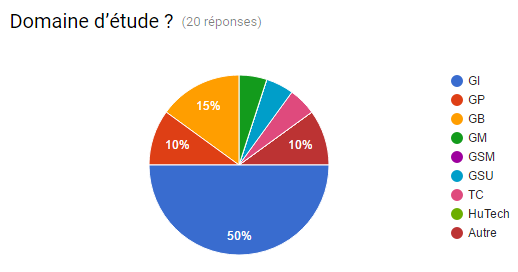
\includegraphics[width=.7\textwidth]{img/sondage_branche}
	\caption{Sondage - Répartition par branches}
\end{figure}
\vspace*{\fill}

On observe que les avis sur les outils déjà existants sont assez mitigés.
En effet, les inconvénients les plus cités sont le manque de personnalisation et le retour en arrière.
D'un autre côté, les avantages cités sont la gratuité et la simplicité d'utilisation.

\newpage
\begin{figure}[!h]
	\centering
	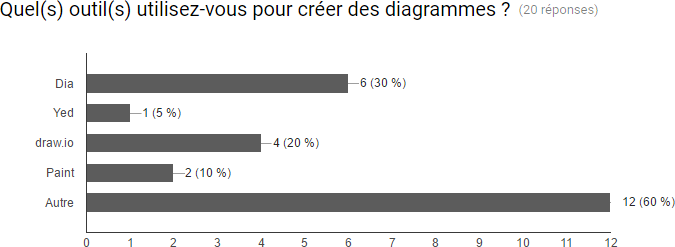
\includegraphics[width=\textwidth]{img/sondage_outils}
	\caption{Sondage - Outils utilisés pour la réalisation de diagrammes}
\end{figure}
\vspace*{\fill}
\begin{figure}[!h]
	\centering
	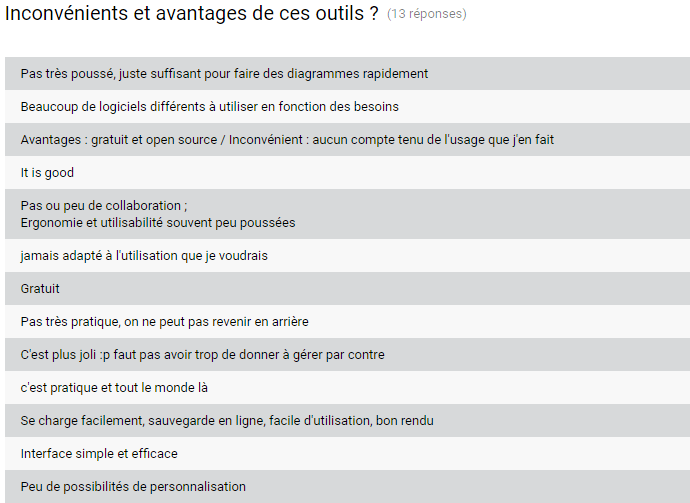
\includegraphics[width=\textwidth]{img/sondage_critique}
	\caption{Sondage - Critiques des outils existants}
\end{figure}
\vspace*{\fill}

\newpage
On peut également voir que les avis quant à l'utilisation d'un appareil mobile pour travailler sont très partagés, on se retrouve à 50\% pour et 50\% contre.
Enfin, l'idée d'une application permettant le travail collaboratif sur appareil mobile est aussi partagée mais tend à pencher pour un avis positif.

\vspace*{\fill}
\begin{figure}[!h]
	\centering
	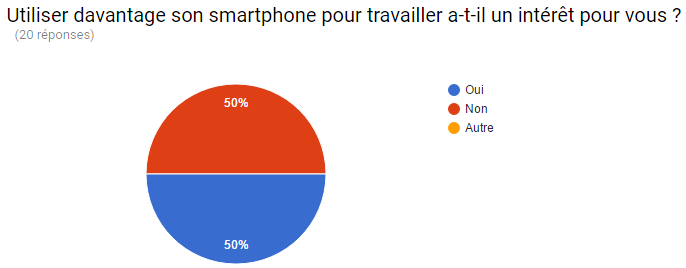
\includegraphics[width=.8\textwidth]{img/sondage_smartphone}
	\caption{Sondage - Critiques des outils existants}
\end{figure}
\vspace*{\fill}
\begin{figure}[h]
	\centering
	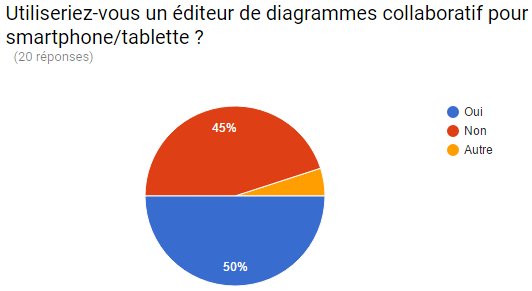
\includegraphics[width=.7\textwidth]{img/sondage_colladia}
	\caption{Sondage - Avis sur Colladia}
\end{figure}
\vspace*{\fill}

\newpage
\subsection{Étude de quelques logiciels concurrents}
Lors de nos recherches, deux applications semblaient réellement en concurrence avec notre solution, à savoir draw.io de Google et DrawExpress de DrawExpress Inc.

\subsubsection{Draw.io}
Néanmoins draw.io, bien que collaboratif n'utilise pas pleinement les fonctionnalités tactiles des supports mobiles.

\vspace*{\fill}
\begin{figure}[h]
	\centering
	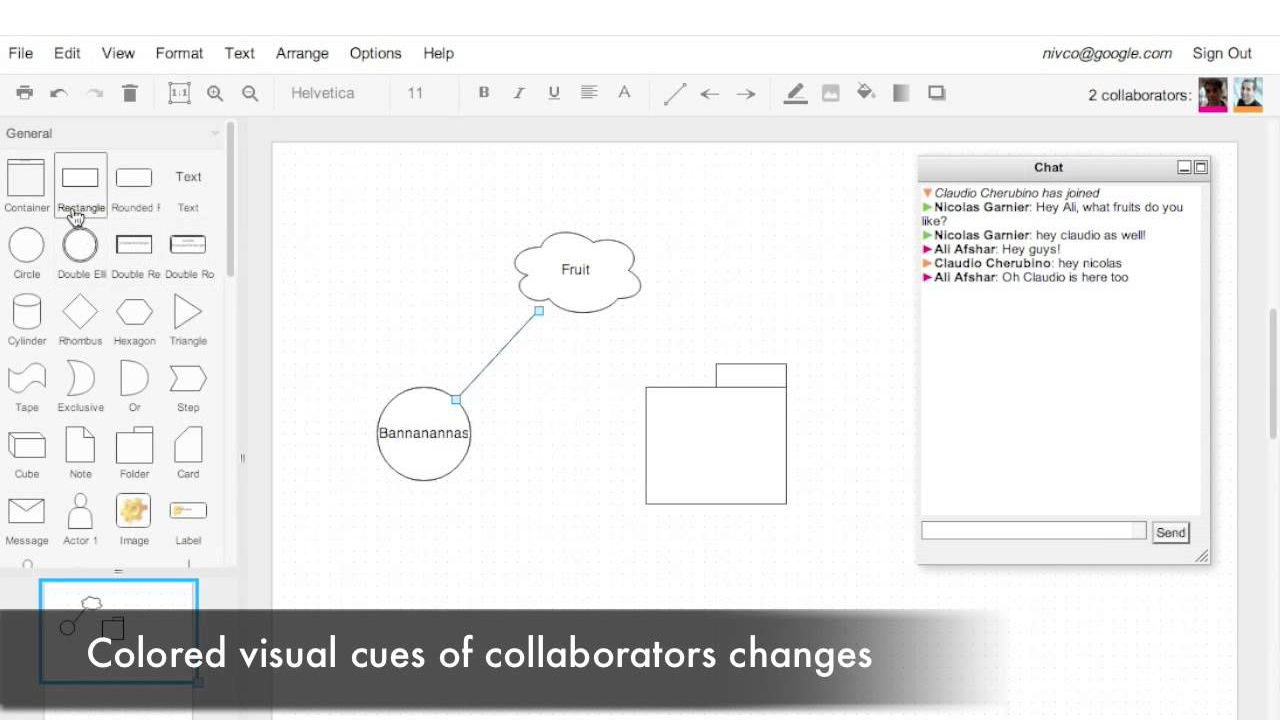
\includegraphics[width=.6\textwidth]{img/drawio}
	\caption{draw.io - Édition en collaboration}
\end{figure}
\vspace*{\fill}

\subsubsection{DrawExpress}
DrawExpress propose un éditeur de diagramme sur mobile.
Il est cross-plateforme (IOS, Android et BlackBerry) mais il ne permet pas de travailler à plusieurs simultanément.

\vspace*{\fill}
\begin{figure}[!h]
	\centering
	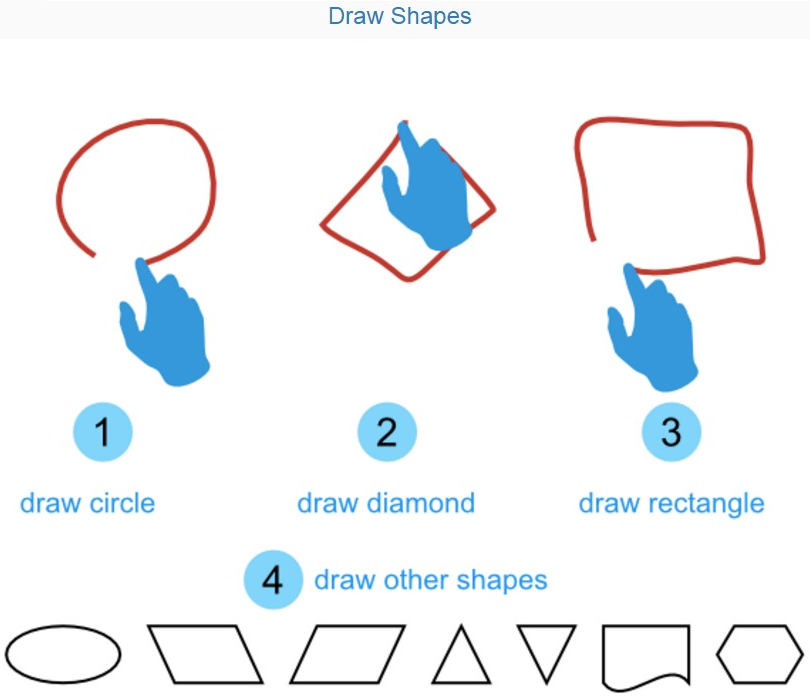
\includegraphics[width=.4\textwidth]{img/DrawExpressRecognition}
	\caption{Aperçu des interactions tactiles de DrawExpress - Reconnaissance de forme}
\end{figure}
\vspace*{\fill}

\newpage
\begin{figure}[!h]
	\centering
	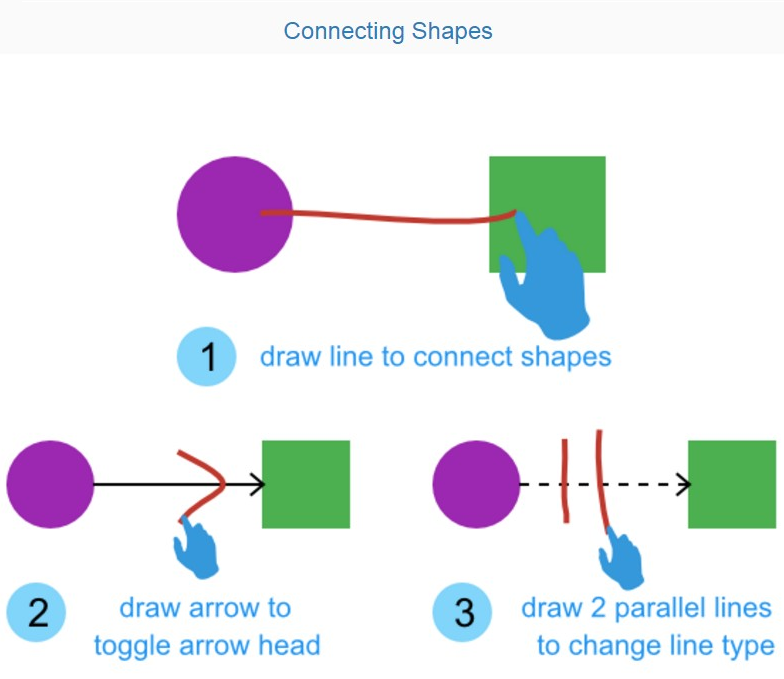
\includegraphics[width=.4\textwidth]{img/DrawExpressLinks}
	\caption{Aperçu des interactions tactiles de DrawExpress - Tracé de lignes}
\end{figure}

Cette application constitue une bonne base d'inspiration pour Colladia puisqu'elle utilise particulièrement les interactions tactiles permises par les smartphones afin de créer, à partir de gestes simples à main levée, des formes prédéfinies qui constituent le diagramme.
De cette manière, l'ergonomie est optimisée pour les écrans tactiles et de petite taille.

\subsubsection{Positionnement}
Le but de Colladia est donc de proposer les deux points forts ces deux logiciels concurrents, à savoir le travail collaboratif et les interactions tactiles.

\newpage
\subsection{Fonctionnalités}
Dans cette partie, on rendra compte des fonctionnalités prévues du cahier des charges, en précisant les modifications qu'elles ont subies lors de leur implémentation.

\subsubsection{Fonctionnalités générales}
	\begin{itemize}
		\item La connexion au serveur avec un pseudo a été correctement réalisée.
		L'utilisateur a la possibilité d'entrer un pseudo et de préciser l'adresse du serveur auquel il faut se connecter pour créer des diagrammes.
		Il lui est aussi permis de sélectionner une couleur personnalisée. 		
		\item Dans la vue listant les diagrammes, il suffit de sélectionner le diagramme voulu et de cliquer sur "Access" pour le rejoindre. Il est aussi possible de supprimer le diagramme.
		
		\vspace*{\fill}
		\begin{figure}[!h]
			\centering
			\begin{subfigure}[t]{.3\textwidth}
				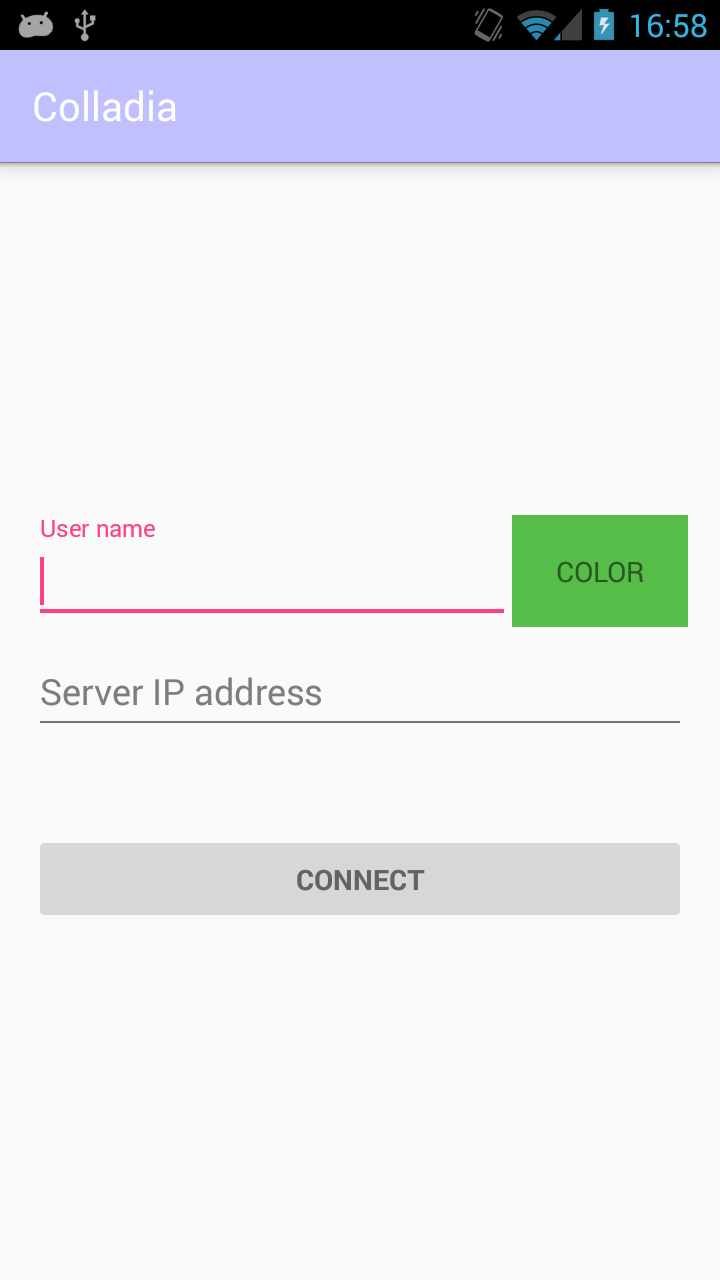
\includegraphics[width=\textwidth]{img/screen/new/colladia_connexion}
				\subcaption{Connexion}
			\end{subfigure}
			~
			\begin{subfigure}[t]{.3\textwidth}
				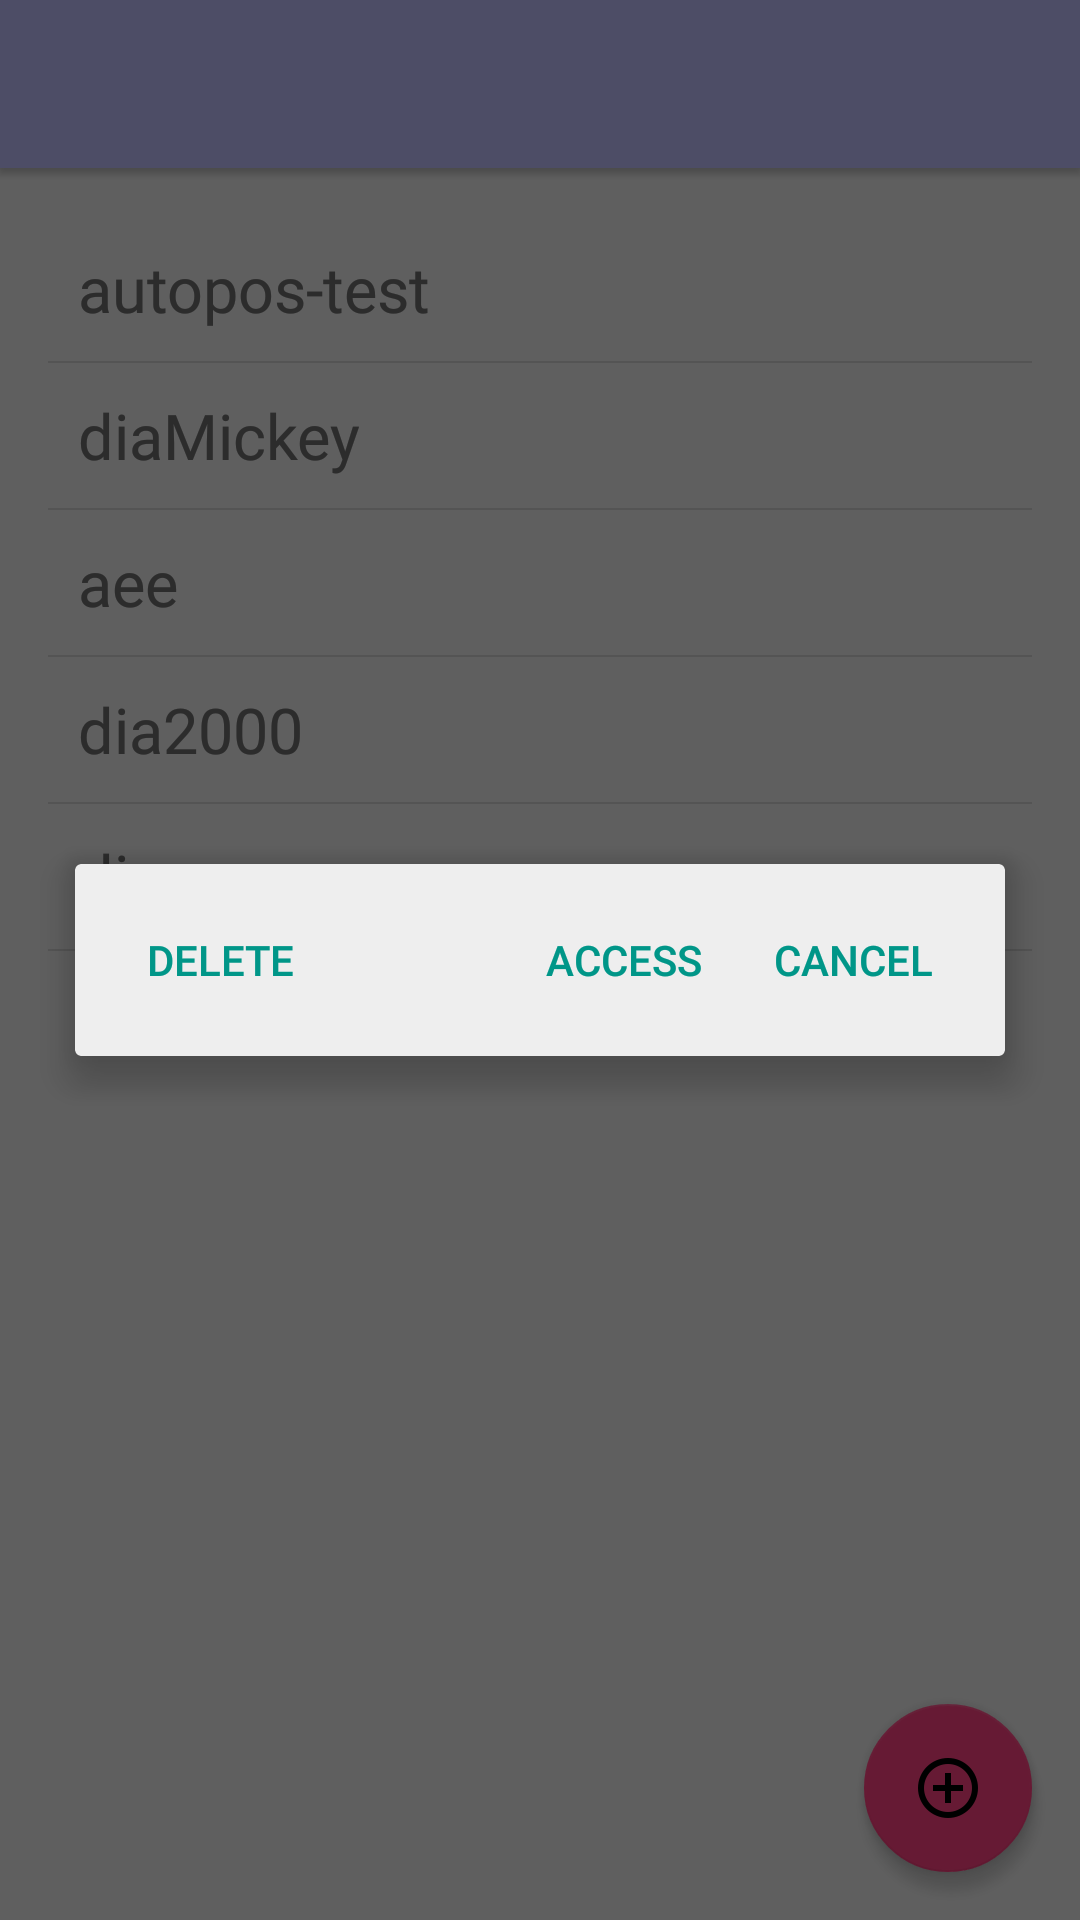
\includegraphics[width=\textwidth]{img/screen/colladia_workspaces_select}
				\subcaption{Liste des diagrammes}
			\end{subfigure}
			~
			\begin{subfigure}[t]{.3\textwidth}
				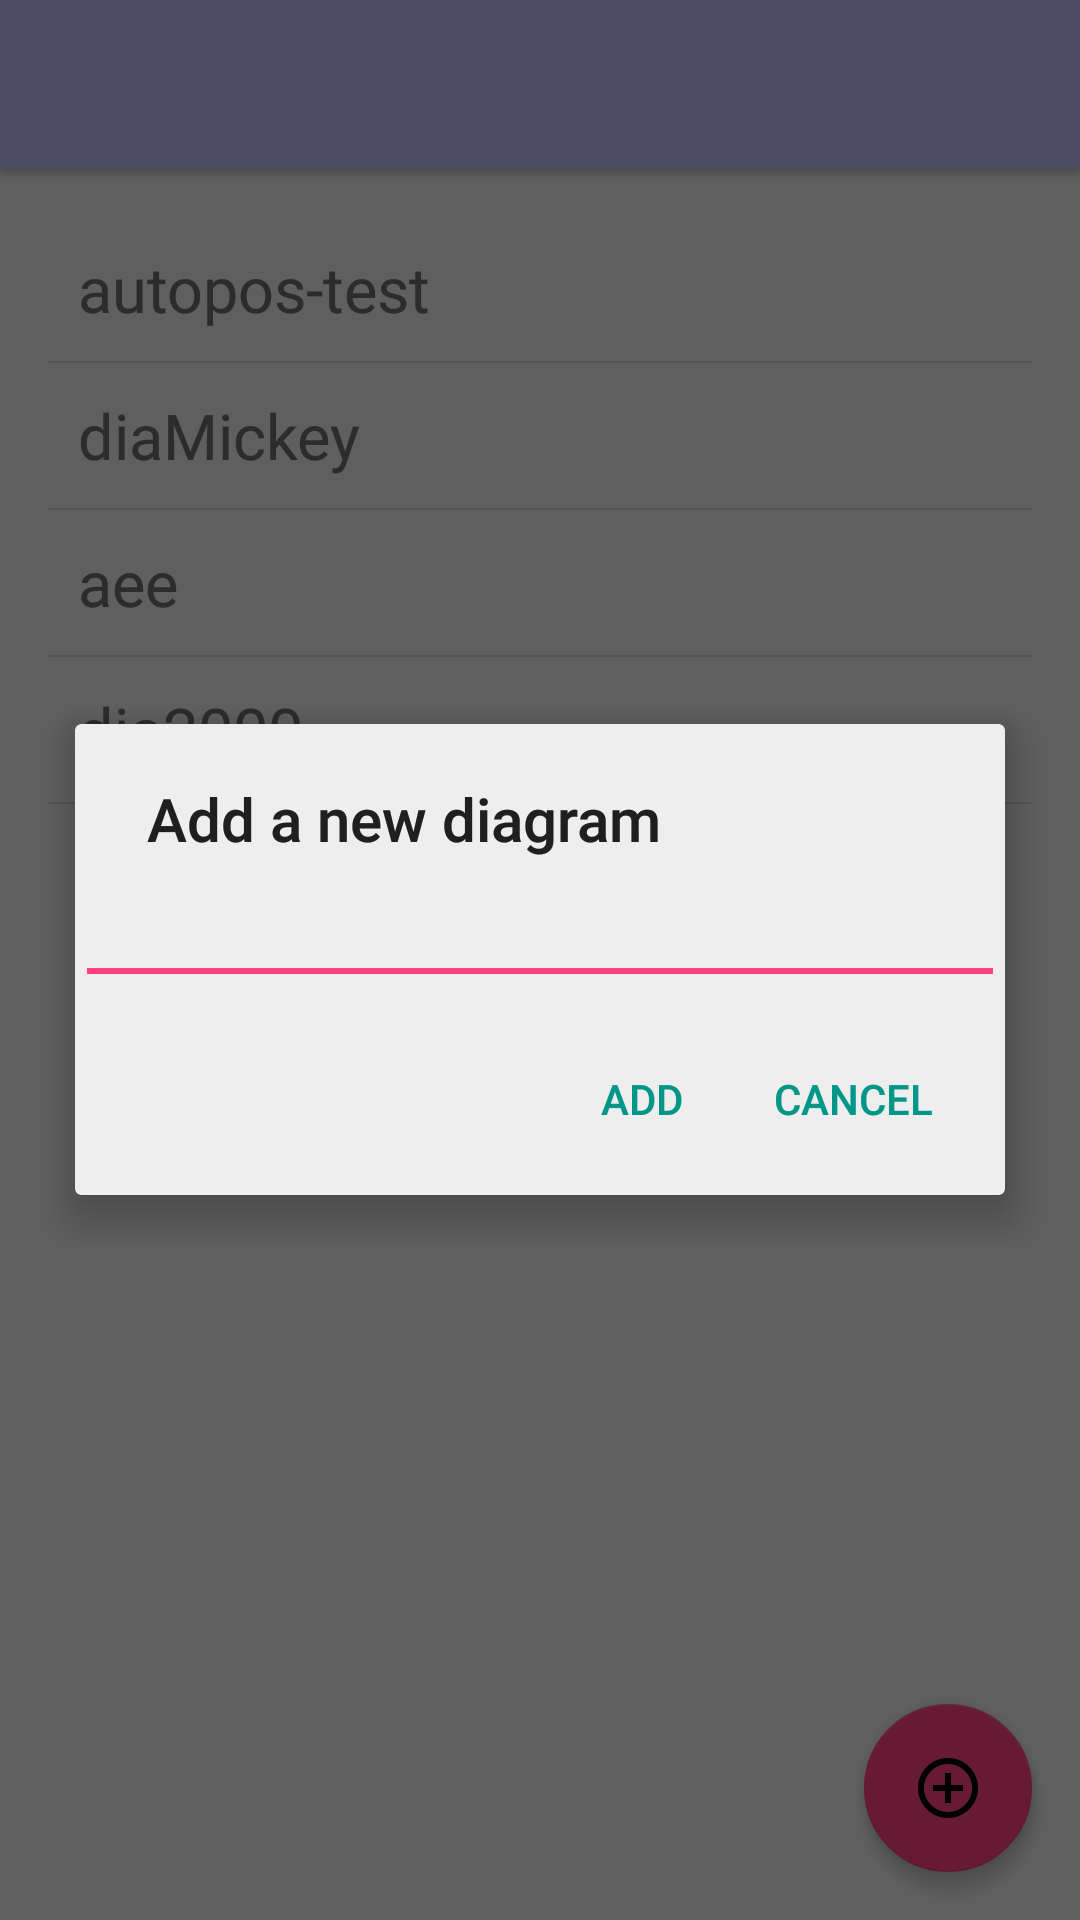
\includegraphics[width=\textwidth]{img/screen/colladia_create_workspace}
				\subcaption{Création}
			\end{subfigure}
			\caption{Colladia - Connexion à l'application et sélection d'un diagramme}
		\end{figure}
		\vspace*{\fill}
		
		\item Inspiré des mouvements de déplacements habituelles sur les interfaces tactiles le mouvement de "swipe" permet de déplacer la vue. Il est aussi possible d'utiliser le mouvement de "pinch" pour effectuer un zoom.
		\item Les fonctionnalités d'ajout, de suppression et de modification d'éléments ont été implémentées et seront détaillées par la suite.
	\end{itemize}
	
\newpage
\subsubsection{Fonctionnalités tactiles implémentées}
\begin{itemize}
\item Icône transparent dans le coin pour ouvrir le menu
\item Ajout de formes prédéfinies (Classes UML, cercles, carrés, rectangles, etc.) en utilisant le menu principal ou le menu contextuel.
\item Un appui long sur un élément permet d'ouvrir un menu contextuel spécifique à l'élément :
\begin{itemize}
	\item pour permettre de supprimer l'élément
	\item pour permettre de dupliquer l'élément
	\item pour permettre de supprimer les liens sortants
\end{itemize}

		\vspace*{\fill}
		\begin{figure}[!h]
			\centering
			\begin{subfigure}[t]{.3\textwidth}
				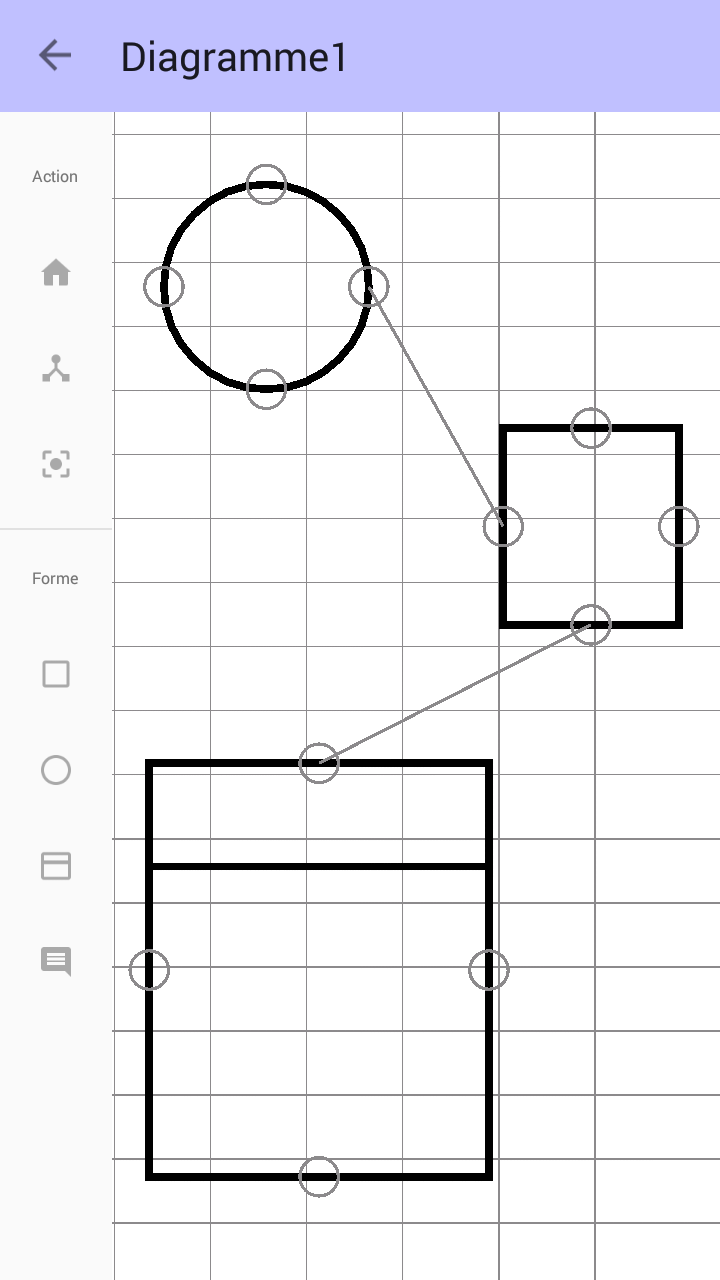
\includegraphics[width=\textwidth]{img/screen/new/colladia_draw_view_menu_main}
				\subcaption{Menu principal}
			\end{subfigure}
			~
			\begin{subfigure}[t]{.3\textwidth}
				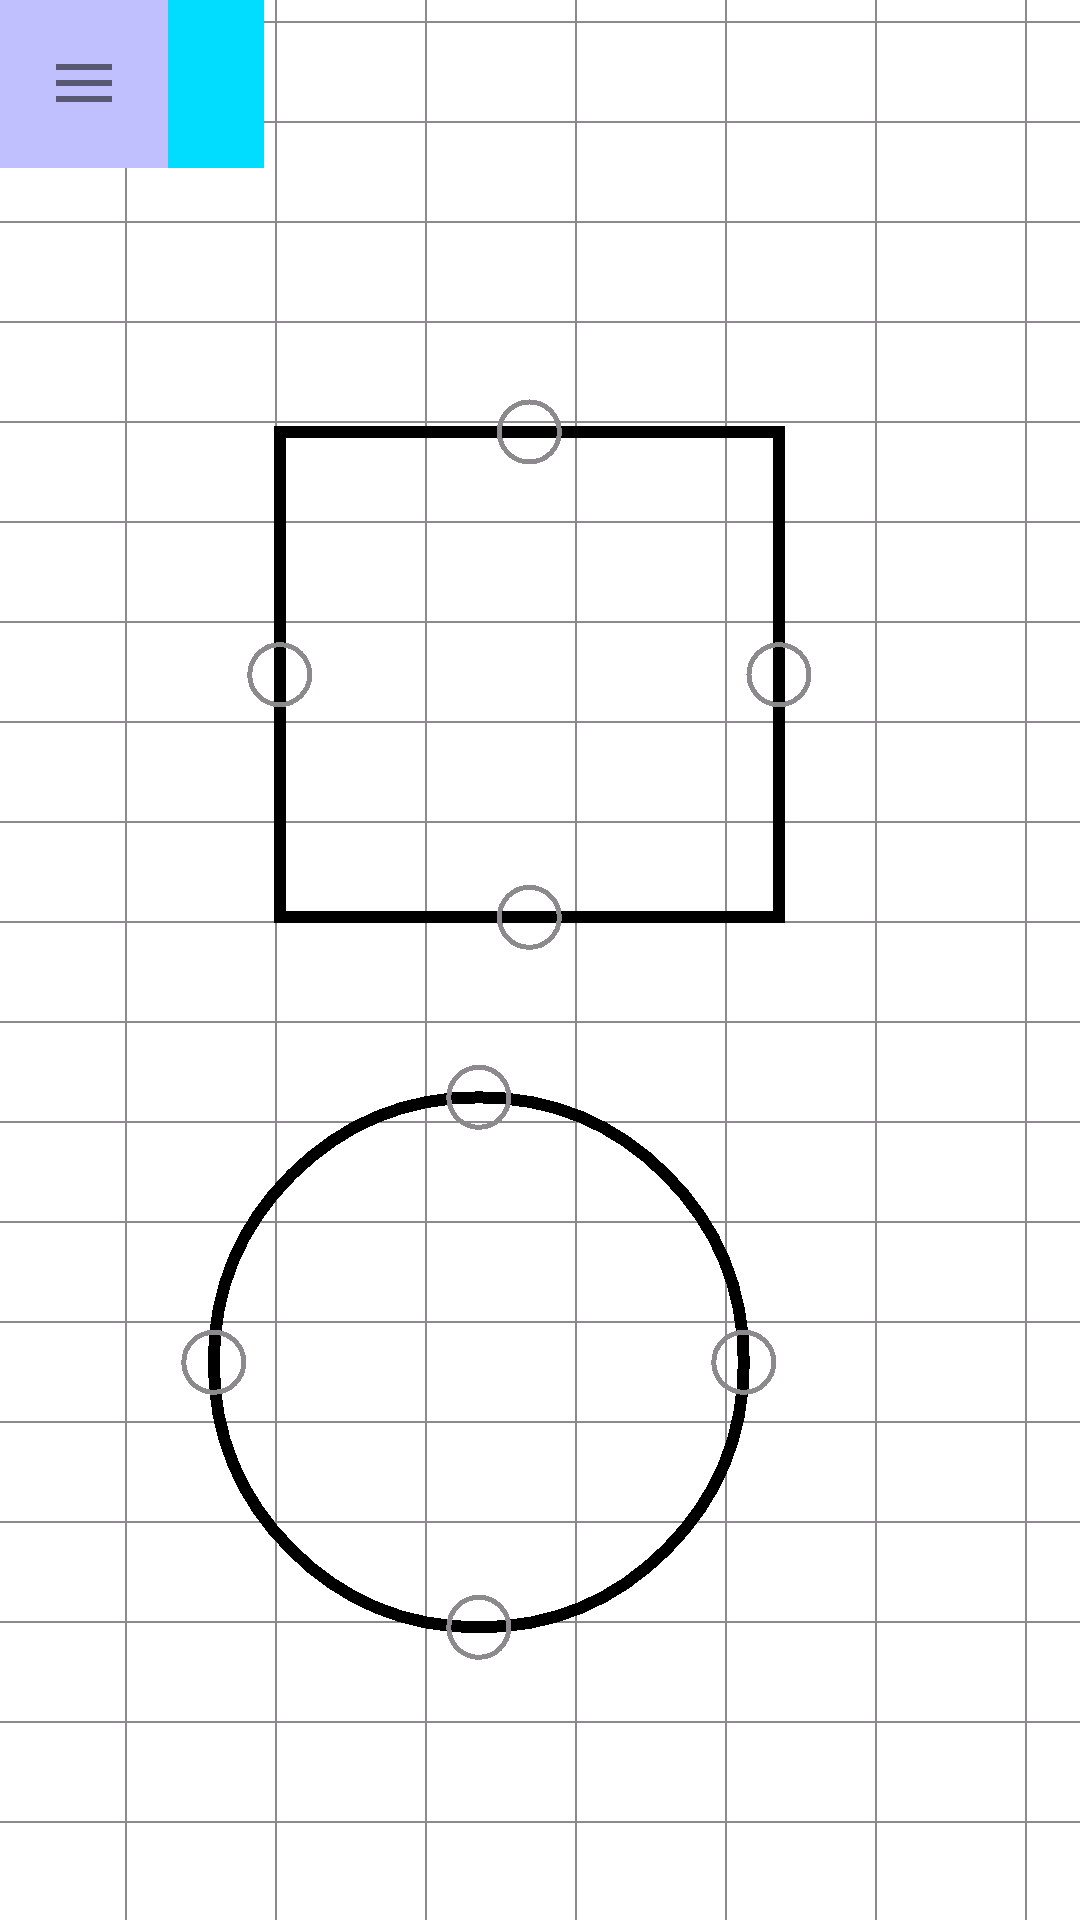
\includegraphics[width=\textwidth]{img/screen/colladia_draw_view_element_2}
				\subcaption{Insertion de formes prédéfinies}
			\end{subfigure}
			~
			\begin{subfigure}[t]{.3\textwidth}
				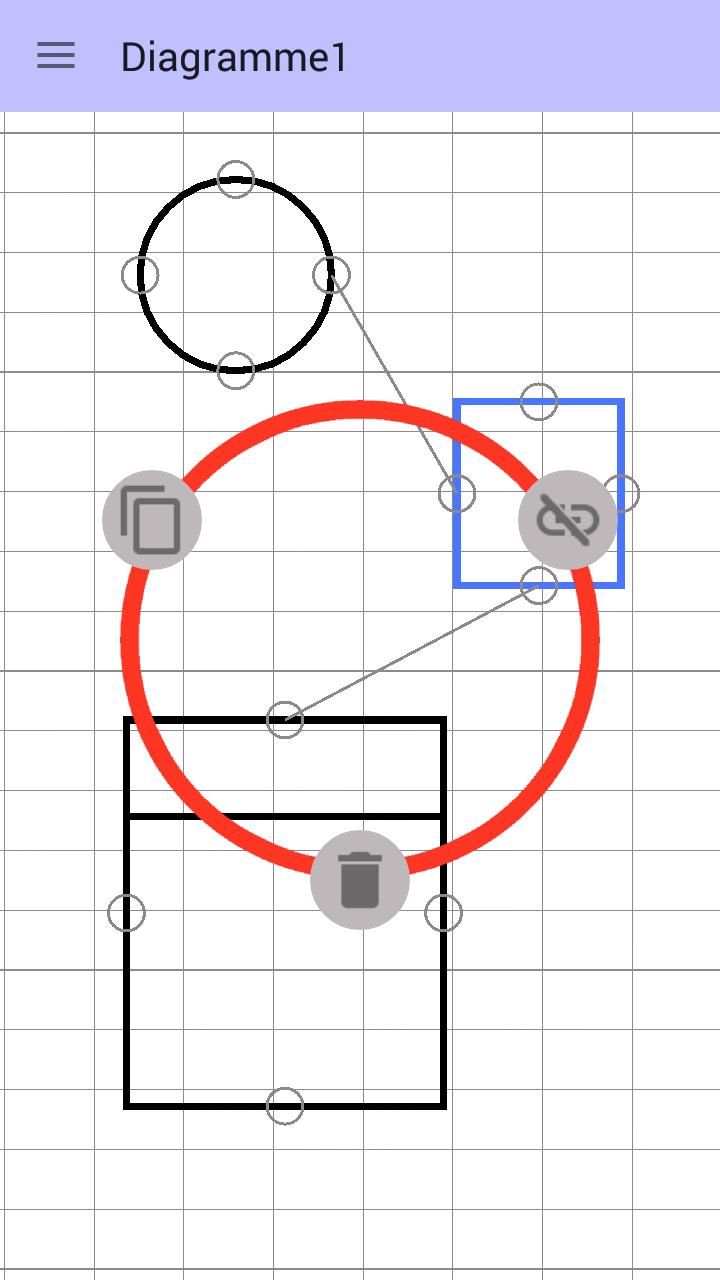
\includegraphics[width=\textwidth]{img/screen/new/colladia_draw_view_menu_contextuel_select}
				\subcaption{Menu contextuel}
			\end{subfigure}
			\caption{Colladia - Menu latéral et menu contextuel}
		\end{figure}
		\vspace*{\fill}
		
\item Un appui long dans le vide permet d'ouvrir un menu pour ajouter des éléments et réaliser des actions :
		\begin{itemize}
			\item Ajout de formes prédéfinies
			\item Repositionner la vue au centre du diagramme
			\item Position automatique des éléments
		\end{itemize}
\item Un "double-tap" sur un élément permet d'insérer du texte dans la forme.
\item Un mouvement de "slide" permet de se déplacer sur la zone de dessin. Si un élément est sélectionné alors on déplace ce dernier.
\item Un appui sur un élément le sélectionne et le colore de la couleur de l'utilisateur. En appuyant de nouveau sur un autre élément ou sur un espace vide, on dé-sélectionne l'élément, et il reprend sa couleur normale.

\newpage
		\begin{figure}[!h]
			\centering
			\begin{subfigure}[t]{.27\textwidth}
				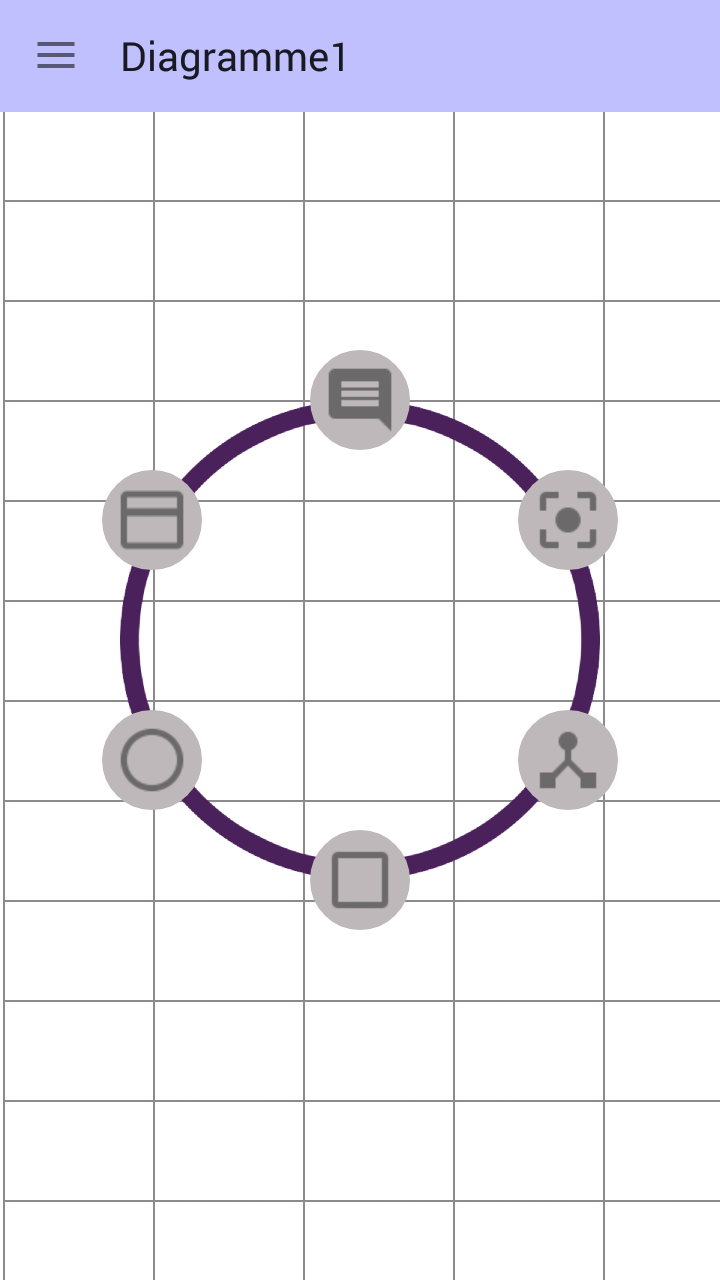
\includegraphics[width=\textwidth]{img/screen/new/colladia_draw_view_menu_contextuel_main}
				\subcaption{Menu contextuel principal}
			\end{subfigure}
			~
			\begin{subfigure}[t]{.27\textwidth}
				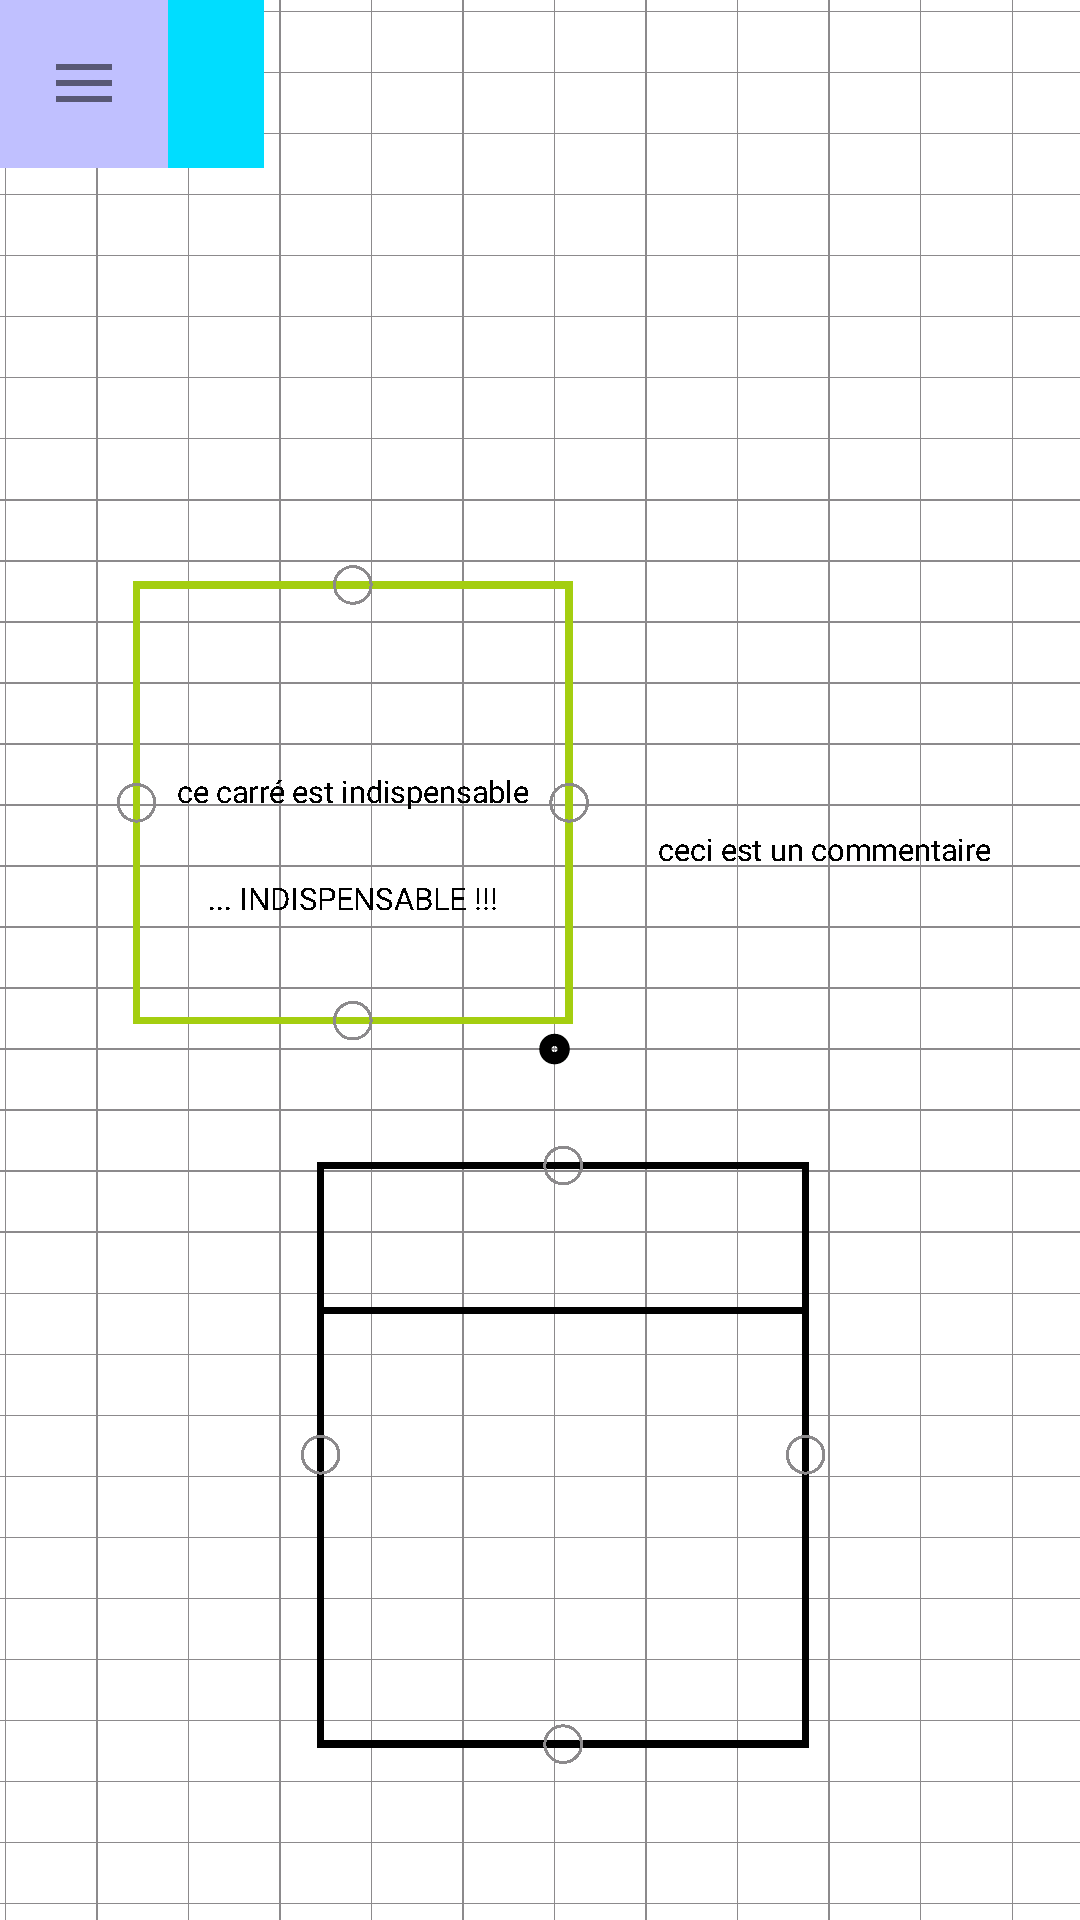
\includegraphics[width=\textwidth]{img/screen/colladia_draw_view_element_text}
				\subcaption{Selection}
			\end{subfigure}
			\caption{Colladia - Menu contextuel principal et sélection d'éléments}
		\end{figure}
		\vspace*{\fill}
		
\item Le mouvement de "pinch" habituel pour gérer les effets de zoom. Si un élément est sélectionné, ce mouvement permet d'effectuer le redimensionnement.
\item Pour pouvoir représenter les flux dans les diagrammes, l'utilisateur peut sélectionner les ancres qui sont au nombre de 4 pour chaque élément, puis en restant appuyé sur l'écran et en rejoignant une seconde ancre un lien sera créée.

	\vspace*{\fill}
		\begin{figure}[!h]
			\centering
			\begin{subfigure}[t]{.27\textwidth}
				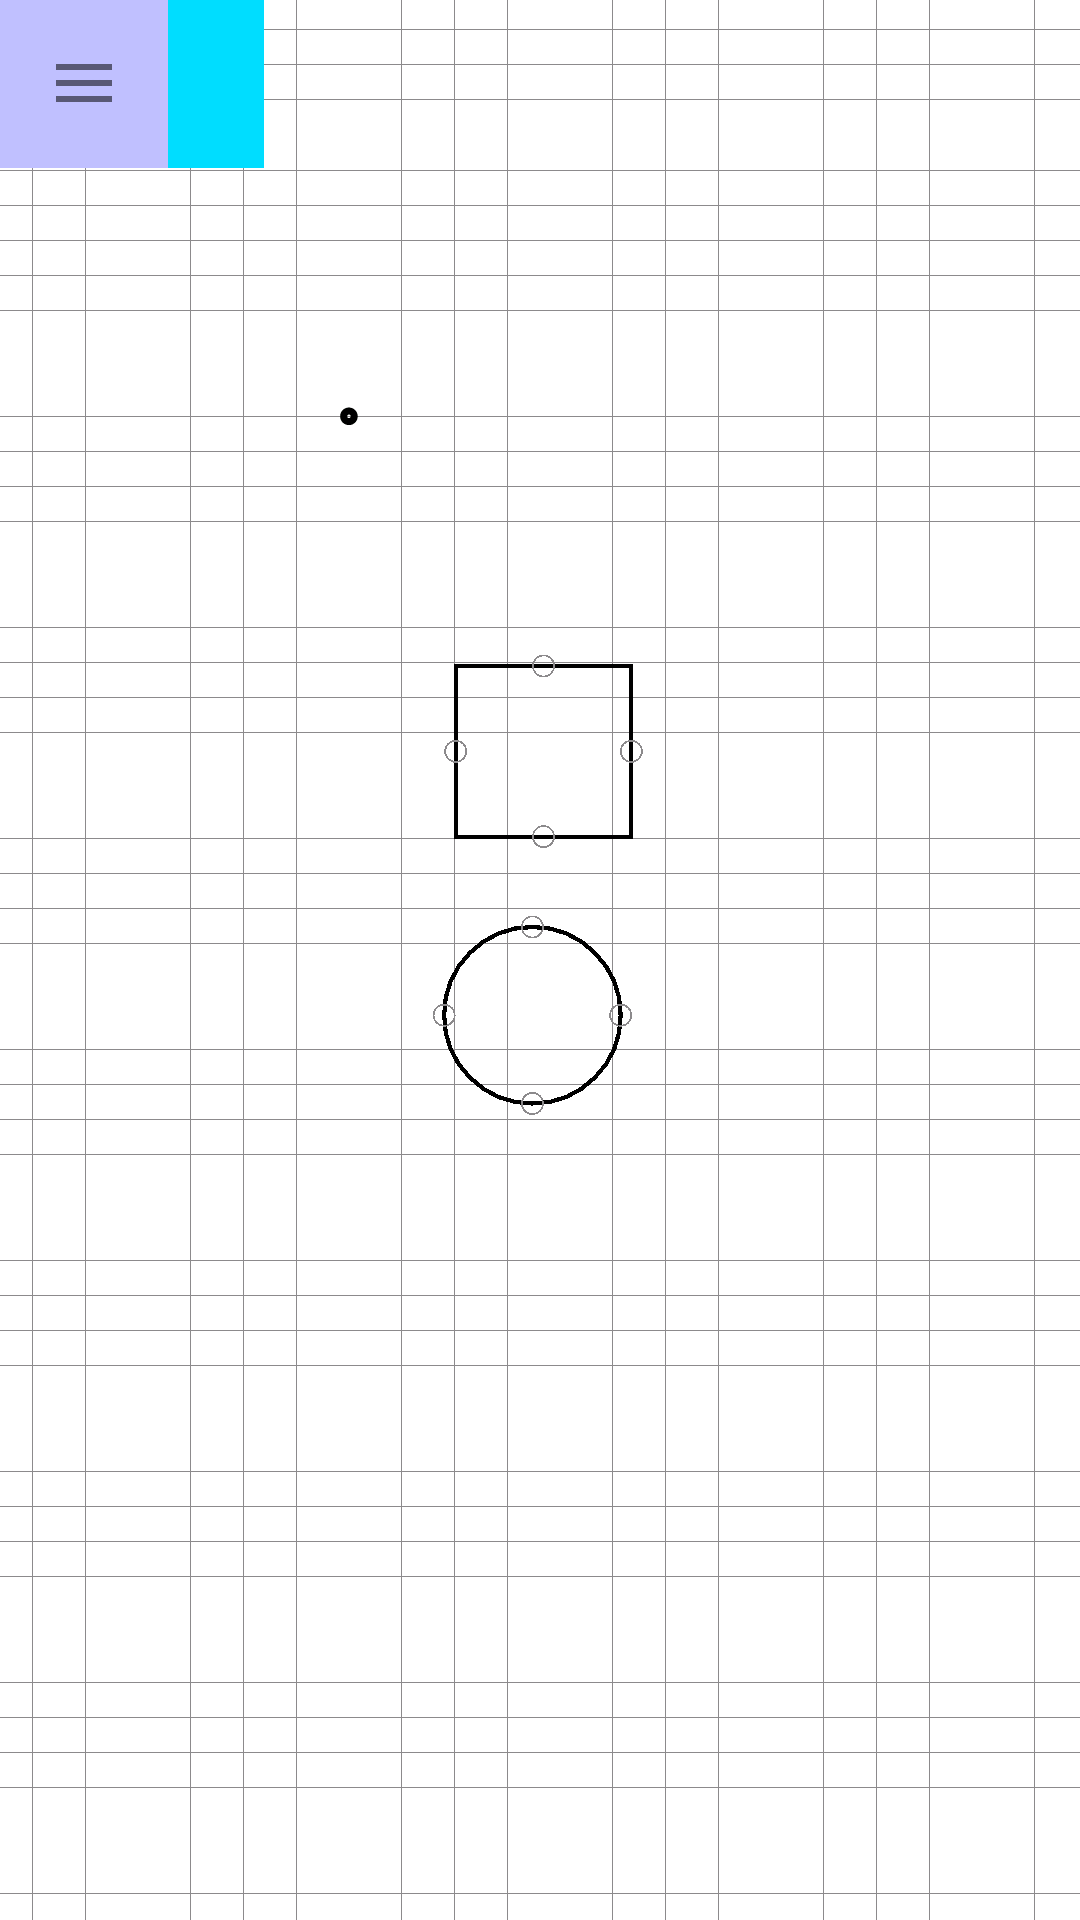
\includegraphics[width=\textwidth]{img/screen/colladia_draw_view_zoom_out}
				\subcaption{Zoom arrière}
			\end{subfigure}
			~
			\begin{subfigure}[t]{.27\textwidth}
				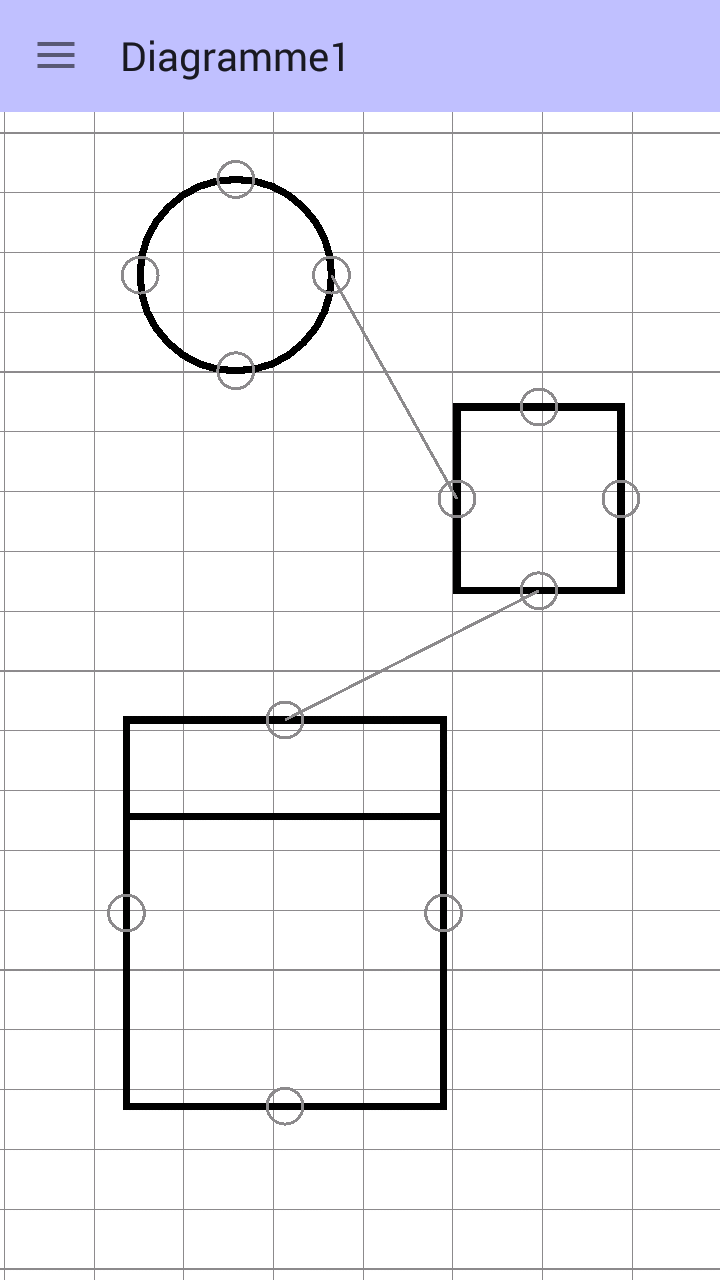
\includegraphics[width=\textwidth]{img/screen/new/colladia_draw_view_element_links}
				\subcaption{Liens}
			\end{subfigure}
			\caption{Colladia - Zoom et liens entre les éléments}
		\end{figure}
\end{itemize}

\newpage
\subsubsection{Fonctionnalités tactiles non-implémentées}
Dans la version actuelle de l'application, la gestion des collaborateurs n'est pas effectuée.
Il n'est donc pas possible de voir les vues des collaborateurs, ni de connaître la liste des utilisateurs connectés à un instant précis.
Néanmoins lorsqu'un élément est sélectionné, il prend la couleur spécifique de l'utilisateur.
Ainsi il est possible de déterminer lorsqu'un item est modifié par un collaborateur. 
La gestion des différents niveaux de plans n'est pas proposé, ainsi que le fait d'attirer l'attention de l'utilisateur sur un élément en particulier, même si cette fonctionnalité est retrouvé lorsque l'on sélectionne l'élément, ce qui la colore. 

\subsubsection{Fonctionnalités tactiles supplémentaires}
Afin de donner une expérience plus intéressante pour l'utilisateur et d'utiliser les capacités du système multi-agents du serveur, il est possible de :
\begin{itemize}
	\item Replacer la vue de l'utilisateur au centre du diagramme pour s'assurer que l'utilisateur puisse toujours se repérer.
	\item Réorganiser l'ensemble des éléments existants en demandant au serveur de replacer les éléments sans que ces derniers ne se chevauchent.
\end{itemize}

\subsubsection{Fonctionnalités optionnelles}
Voici les fonctionnalités optionnelles pour améliorer l'expérience utilisateur qui avaient été proposées au début du projet :
\begin{itemize}
\item un chat pour laisser la possibilité aux membres de communiquer
\item l'utilisation de commandes vocales pour faciliter l'utilisation de l'application
\item un système de commentaire sur les diagrammes, pour fournir des informations complémentaires
\item une fonction de recherche de texte
\item la fusion de diagrammes
\item l'exportation des diagrammes sous différents formats (graphml par exemple)
\item la gestion des utilisateurs
\item la possibilité de restreindre l'accès à un diagramme par un mot de passe
\item la gestion des sauvegardes hors-ligne
\item le dessin à main levé qui permet une reconnaissance de forme et d'ajout d'élément automatiquement
\end{itemize}

Parmi ces dernières la gestion des sauvegardes automatiques côté serveur a été implémenté, en sauvegardant dans des fichiers les diagrammes sous format JSON. Les diagrammes sont donc persistants et accessibles d'une utilisation à l'autre.

\newpage
\subsection{Technologies}
Concernant les technologies employées, le serveur utilise la plateforme multi-agent JADE et communique avec le client via une API Restlet.
Côté client il avait été envisagé de réaliser l'application en utilisant Xamarin dans un premier temps, néanmoins la technologie ne fonctionnait pas correctement chez tous les membres du projet.
Il a fallu réagir et prendre une décision pour pouvoir réaliser le projet dans le délai imparti.
Le choix a été pris de réaliser l'application en Android natif, ce qui permet d'avoir accès à une documentation importante et d'avoir une application réactive.
\vspace*{-.5cm}

\subsection{Architecture de l'application}
L'application cliente est constituée de 3 vues principales, qui s'occupent de l'essentiel des interactions avec l'utilisateur.
Elles permettent de gérer les entrées d'utilisateurs.
La première vue gère la connexion au serveur avec la création des données utilisateurs. Lors de la connexion, la deuxième vue est affichée pour lister les diagrammes existants et en créer de nouveau.
Une fois un diagramme sélectionné, la dernière vue est affichée pour permettre d'éditer le diagramme. 
	
 	\vspace*{\fill}
	\begin{figure}[!h]
		\centering
		\includegraphics[width=.7\textwidth]{img/FlowAppli}
		\caption{Colladia - Vues principales}
	\end{figure}
 	\vspace*{\fill}
\vspace*{-.5cm}

\subsubsection{Architecture Général}
L'application peut-être schématisée comme suit, à savoir le contrôleur situé entre la vue et le modèle. Dès qu'une modification est effectuée au niveau de la liste des éléments du modèle le contrôleur met à jour la vue.
Dans le sens contraire lorsque l'utilisateur interagit avec la vue une requête est envoyé au serveur pour mette à jour le diagramme sur le serveur pour les autres utilisateurs.
Le modèle est mis à jour par le serveur par le retour d'une requête de modification ou par la réponse d'une requête GET qui est réalisé périodiquement pour savoir si de nouvelles modifications sont présentes sur le serveur.

 	\vspace*{\fill}
	\begin{figure}[!h]
		\centering
		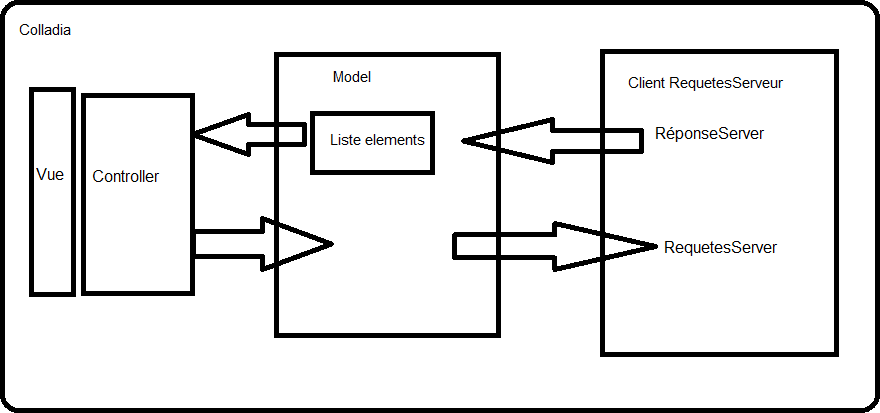
\includegraphics[width=.6\textwidth]{img/archiGeneral}
		\caption{Colladia - Schéma de l'architecture général}
	\end{figure}
 	\vspace*{\fill}
	
\newpage
\subsubsection{Structure de données}
Outre les données utilisateur, les structures de données principales concernent les éléments.
Pour pouvoir proposer de nombreuses formes prédéfinis, il a été décidé de créer une classe Element abstraite dont hériteraient toutes les formes.
Ainsi le contrôleur peut gérer les éléments sans avoir à connaître le type d'élément dont il s'agit.
Ce polymorphisme induit un couplage plus léger et permet donc une plus grande souplesse du contrôleur.
Certaines méthodes telles que \lstinline$isTouch(PointF indexUser)$ qui permet de savoir si un élément a été touché par l'index de l'utilisateur ou \lstinline$draw()$ qui permet de dessiner l'élément.
En surchargeant ces différentes méthodes chaque forme peut proposer un comportement différent.
Les éléments se distinguent entre eux par le stockage d'un identifiant \lstinline$UUID$ qui est unique, ce qui permet de sérialiser/dé-sérialiser sous format JSON les objets puis retrouver leurs références. 

	\vspace*{\fill}
	\begin{figure}[!h]
		\centering
		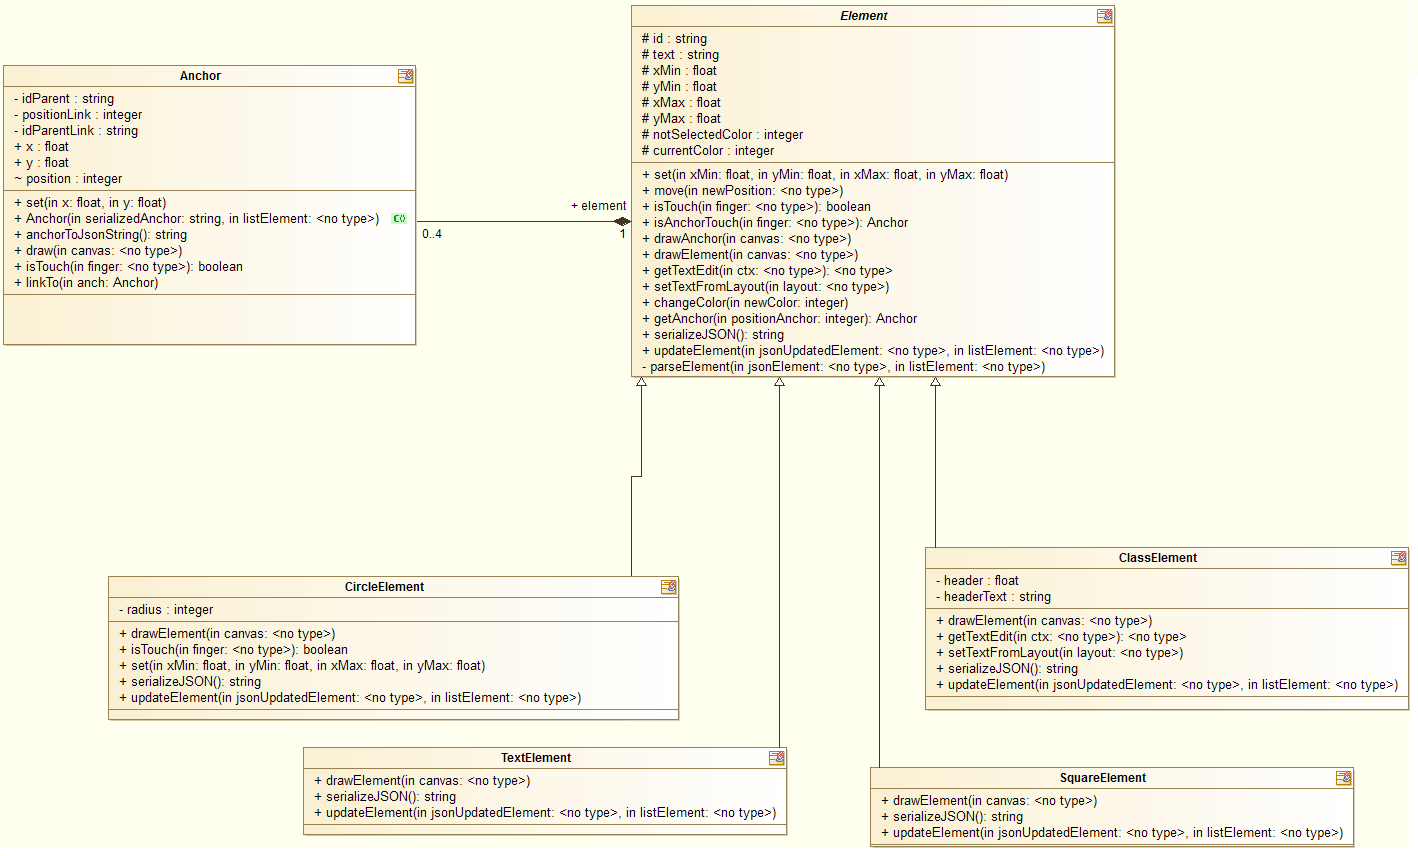
\includegraphics[width=\textwidth]{img/UmlArchiStructureData}
		\caption{Colladia - Structure de données simplifiée}
	\end{figure}
	\vspace*{\fill}
	
Chaque élément possède 4 ancres (Top, Bottom, Left, Right) qui permettent de lier les éléments entre eux.
Pour ce faire chaque ancre possède l'UUID de son parent ainsi que celui de l'ancre auquel il est associé.
Lors de la sérialisation/dé-sérialisation des éléments il est possible de retrouver l'ancre associée sans pour autant avoir une référence sur l'objet constamment.
\vspace*{\fill}

\newpage
\subsubsection{Gestion des données}
Le singleton \lstinline$Manager$ propose des méthodes telles que \lstinline$changeText(Element elmnt, Text text)$ qui permet dans un premier temps de changer le texte l'élément, puis demande au \lstinline$Requestator$ d'envoyer une requête au serveur pour y mettre à jour l'élément.
Le singleton \lstinline$Requestator$ s'occupe de réaliser les requêtes au serveur en utilisant le framework android Volley.
Le modèle possède le diagramme couramment modifié ainsi que l'horloge logique utilisé par le serveur pour renvoyer les dernières modifications effectuées.

	\begin{figure}[!h]
		\centering
		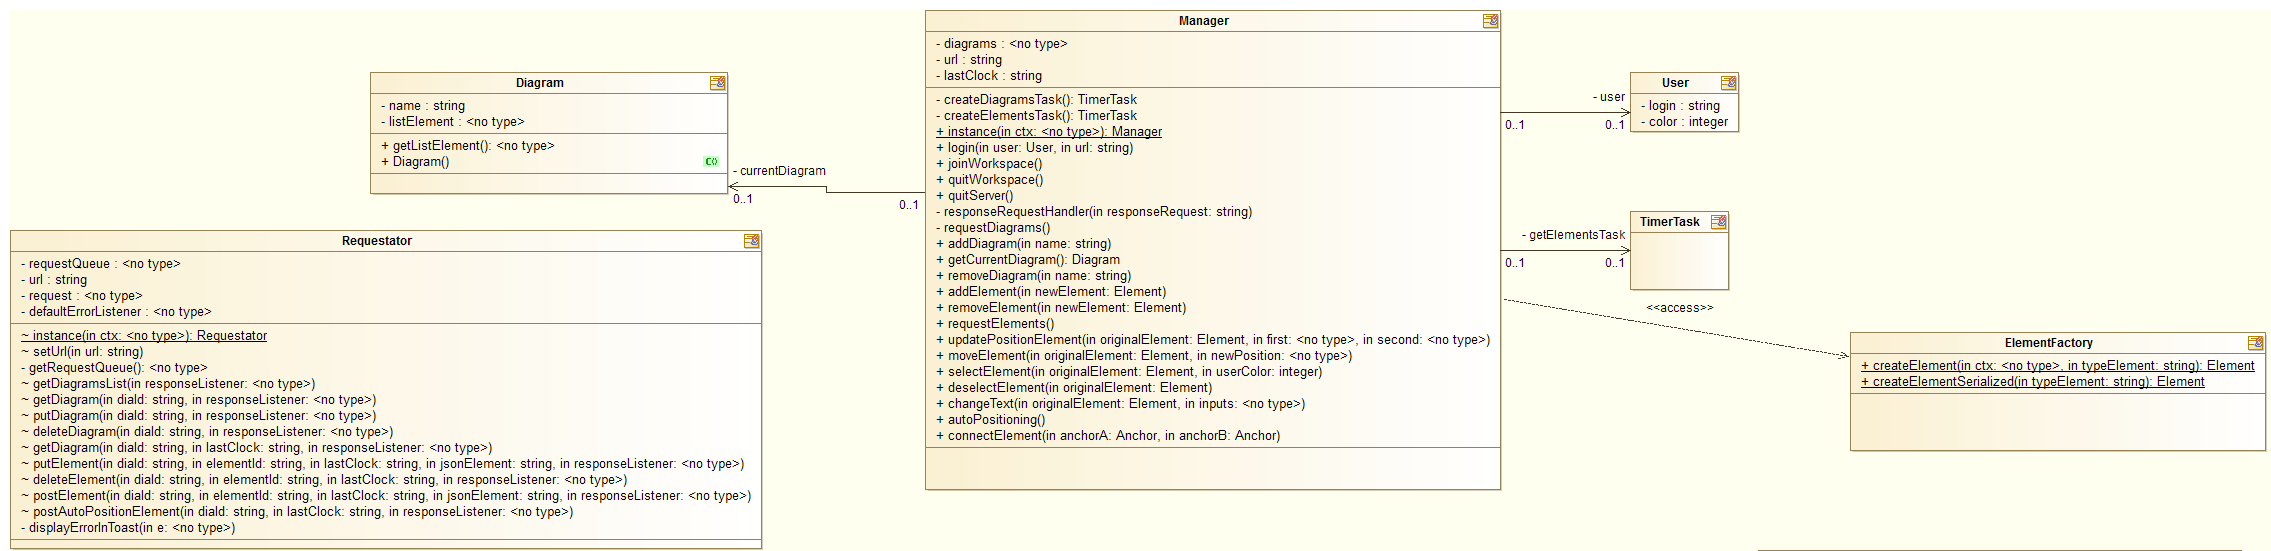
\includegraphics[width=\textwidth]{img/UmlArchiGeneral}
		\caption{Colladia - Gestion des données simplifiée}
	\end{figure}
	
La classe \lstinline$ElementFactory$ permet de générer les éléments spécifiques tels un Cercle ou un Rectangle pour les proposer au Manager qui via le polymorphisme traitera l'objet comme un simple \lstinline$Element$.

\subsubsection{Différentes vues}
On retrouve le concept du MVC au niveau des différentes vues que ce soit au niveau de la connexion au serveur avec les données utilisateur, mais aussi avec la liste des diagrammes qui met à jour automatiquement la vue lorsqu'une modification arrive du serveur et modifie le modèle. Le design pattern Observable était une nécessité dans le contexte asynchrone de requêtage HTTP.

% \paragraph{Édition d'un diagramme}
Concernant la zone de dessin il a fallu mettre en place une sorte de machine à états qui changerait de "mode" selon les interactions de l'utilisateur. Il existe différents modes (\lstinline$ZOOM$, \lstinline$SCROLL$, \lstinline$INSERT$, ...), ce qui permet de déterminer le comportement à adopter selon la situation rencontrée.

La méthode \lstinline$onTouchEvent()$ réagit aux différentes interactions de l'utilisateur, puis appelle la méthode adéquate comme par exemple \lstinline$moveTouch()$ qui correspond au déplacement du doigt de l'utilisateur sur l'écran.  

\newpage
	\begin{figure}[!h]
		\centering
		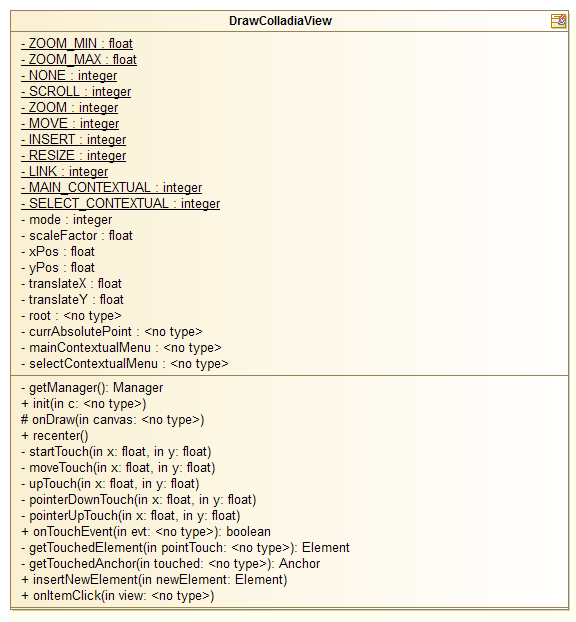
\includegraphics[width=.8\textwidth]{img/UmlDrawView}
		\caption{Colladia - DrawColladiaView}
	\end{figure}

\subsection{Limites et améliorations}
L'application possède une base intéressante et fonctionnelle, cependant on peut citer quelques limites principales.
La première limite étant le nombre restreint d'éléments différents qui sont actuellement proposés.
Un travail important été réalisé pour factoriser un maximum de code des éléments au niveau de la classe \lstinline$Element$, ce qui permet de créer assez facilement des formes diverses et variés.
Une des fonctionnalités supplémentaires qui pourrait aider l'utilisateur serait de permettre une sélection groupée, en plus des différentes fonctionnalités optionnelles décrites auparavant. 
